% Options for packages loaded elsewhere
\PassOptionsToPackage{unicode}{hyperref}
\PassOptionsToPackage{hyphens}{url}
%
\documentclass[
  ignorenonframetext,
]{beamer}
\usepackage{pgfpages}
\setbeamertemplate{caption}[numbered]
\setbeamertemplate{caption label separator}{: }
\setbeamercolor{caption name}{fg=normal text.fg}
\beamertemplatenavigationsymbolsempty
% Prevent slide breaks in the middle of a paragraph
\widowpenalties 1 10000
\raggedbottom
\setbeamertemplate{part page}{
  \centering
  \begin{beamercolorbox}[sep=16pt,center]{part title}
    \usebeamerfont{part title}\insertpart\par
  \end{beamercolorbox}
}
\setbeamertemplate{section page}{
  \centering
  \begin{beamercolorbox}[sep=12pt,center]{part title}
    \usebeamerfont{section title}\insertsection\par
  \end{beamercolorbox}
}
\setbeamertemplate{subsection page}{
  \centering
  \begin{beamercolorbox}[sep=8pt,center]{part title}
    \usebeamerfont{subsection title}\insertsubsection\par
  \end{beamercolorbox}
}
\AtBeginPart{
  \frame{\partpage}
}
\AtBeginSection{
  \ifbibliography
  \else
    \frame{\sectionpage}
  \fi
}
\AtBeginSubsection{
  \frame{\subsectionpage}
}
\usepackage{amsmath,amssymb}
\usepackage{iftex}
\ifPDFTeX
  \usepackage[T1]{fontenc}
  \usepackage[utf8]{inputenc}
  \usepackage{textcomp} % provide euro and other symbols
\else % if luatex or xetex
  \usepackage{unicode-math} % this also loads fontspec
  \defaultfontfeatures{Scale=MatchLowercase}
  \defaultfontfeatures[\rmfamily]{Ligatures=TeX,Scale=1}
\fi
\usepackage{lmodern}
\usetheme[]{Boadilla}
\ifPDFTeX\else
  % xetex/luatex font selection
\fi
% Use upquote if available, for straight quotes in verbatim environments
\IfFileExists{upquote.sty}{\usepackage{upquote}}{}
\IfFileExists{microtype.sty}{% use microtype if available
  \usepackage[]{microtype}
  \UseMicrotypeSet[protrusion]{basicmath} % disable protrusion for tt fonts
}{}
\makeatletter
\@ifundefined{KOMAClassName}{% if non-KOMA class
  \IfFileExists{parskip.sty}{%
    \usepackage{parskip}
  }{% else
    \setlength{\parindent}{0pt}
    \setlength{\parskip}{6pt plus 2pt minus 1pt}}
}{% if KOMA class
  \KOMAoptions{parskip=half}}
\makeatother
\usepackage{xcolor}
\newif\ifbibliography
\usepackage{longtable,booktabs,array}
\usepackage{calc} % for calculating minipage widths
\usepackage{caption}
% Make caption package work with longtable
\makeatletter
\def\fnum@table{\tablename~\thetable}
\makeatother
\usepackage{graphicx}
\makeatletter
\def\maxwidth{\ifdim\Gin@nat@width>\linewidth\linewidth\else\Gin@nat@width\fi}
\def\maxheight{\ifdim\Gin@nat@height>\textheight\textheight\else\Gin@nat@height\fi}
\makeatother
% Scale images if necessary, so that they will not overflow the page
% margins by default, and it is still possible to overwrite the defaults
% using explicit options in \includegraphics[width, height, ...]{}
\setkeys{Gin}{width=\maxwidth,height=\maxheight,keepaspectratio}
% Set default figure placement to htbp
\makeatletter
\def\fps@figure{htbp}
\makeatother
\setlength{\emergencystretch}{3em} % prevent overfull lines
\providecommand{\tightlist}{%
  \setlength{\itemsep}{0pt}\setlength{\parskip}{0pt}}
\setcounter{secnumdepth}{-\maxdimen} % remove section numbering
\usepackage{graphicx}
\logo{\ifnum\thepage>1\hfill
\includegraphics[width=1cm]{logo}\fi}
\titlegraphic{
\includegraphics[width=3cm]{logo}}
\ifLuaTeX
  \usepackage{selnolig}  % disable illegal ligatures
\fi
\usepackage{bookmark}
\IfFileExists{xurl.sty}{\usepackage{xurl}}{} % add URL line breaks if available
\urlstyle{same}
\hypersetup{
  pdftitle={Descriptive Statistics},
  pdfauthor={Pablo E. Gutierrez-Fonseca},
  hidelinks,
  pdfcreator={LaTeX via pandoc}}

\title{Descriptive Statistics}
\author{Pablo E. Gutierrez-Fonseca}
\date{Fall 2024}

\begin{document}
\frame{\titlepage}

\begin{frame}{Why describe data?}
\phantomsection\label{why-describe-data}
\begin{itemize}
\tightlist
\item
  Determine if our sample reflects the population of interest.
\end{itemize}

\begin{itemize}
\tightlist
\item
  Identify outliers.
\end{itemize}

\begin{itemize}
\tightlist
\item
  Obtain metrics necessary for inferential tests.
\end{itemize}

\begin{itemize}
\tightlist
\item
  Understand the distribution of our data values -- test for normality.
\end{itemize}

\begin{itemize}
\tightlist
\item
  Identify the type of statistical test to run.
\end{itemize}
\end{frame}

\begin{frame}{Data description and visualization}
\phantomsection\label{data-description-and-visualization}
\begin{itemize}
\tightlist
\item
  We can examine our data and run statistical tests to see if the
  distribution approximates a normal curve.\\
\item
  Typically, we start by visualizing our data.
\end{itemize}

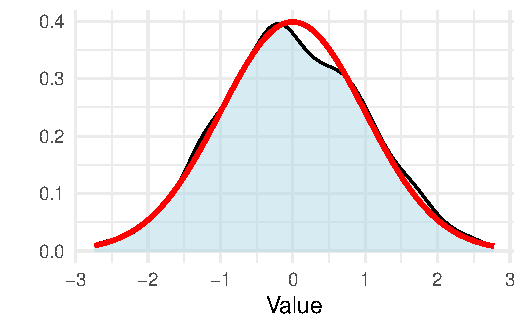
\includegraphics{M4-Descriptice-Statistics_files/figure-beamer/unnamed-chunk-1-1.pdf}
\end{frame}

\begin{frame}{Histogram basic}
\phantomsection\label{histogram-basic}
\begin{itemize}
\tightlist
\item
  Continuous data are most commonly visualized using Histograms.
\end{itemize}

\begin{figure}
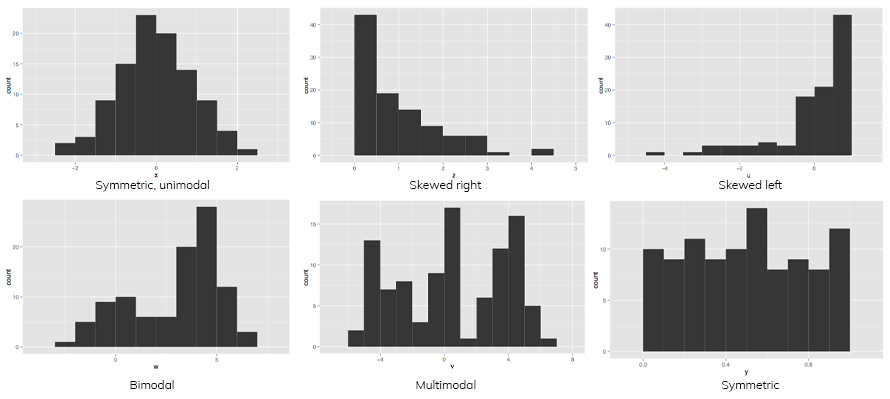
\includegraphics[width=0.8\linewidth]{fig/Histogram} \end{figure}
\end{frame}

\begin{frame}{Box and Whisker Basics}
\phantomsection\label{box-and-whisker-basics}
\begin{figure}
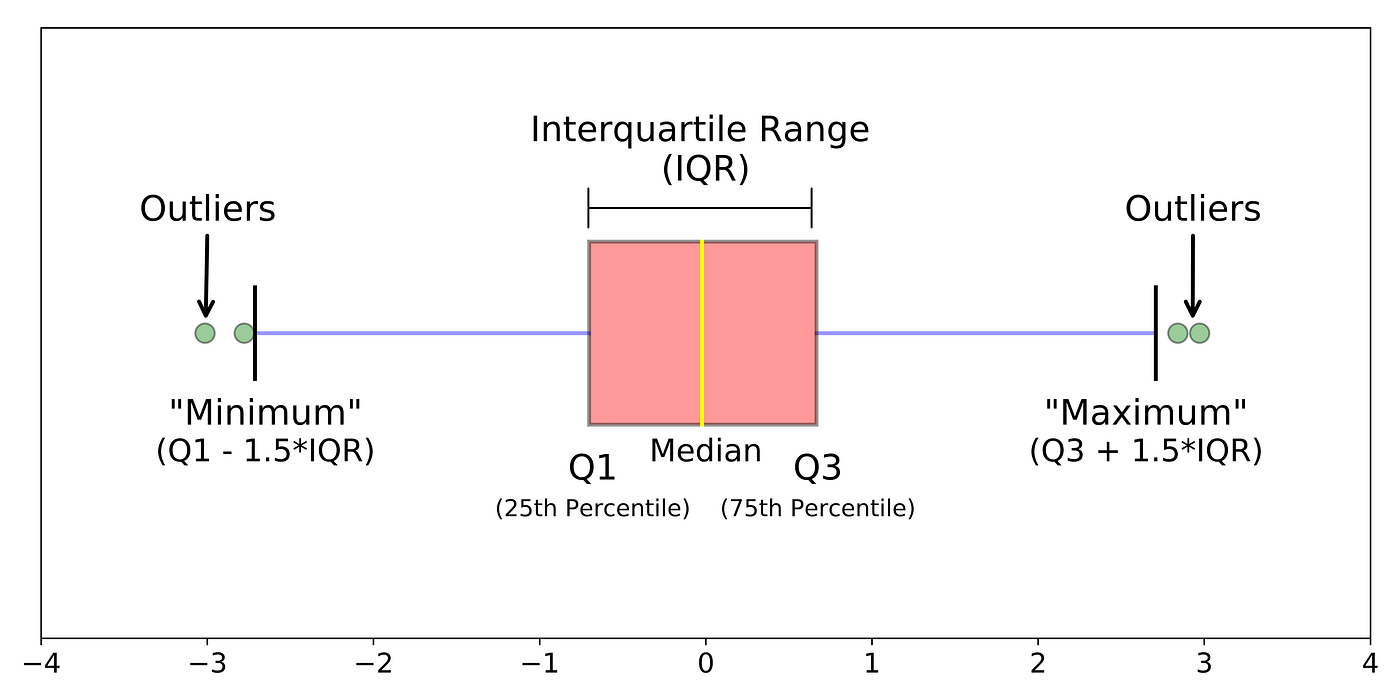
\includegraphics[width=0.8\linewidth]{fig/box} \end{figure}
\end{frame}

\begin{frame}{Metrics to Describe data distribution.}
\phantomsection\label{metrics-to-describe-data-distribution.}
\begin{itemize}
\item
  Data and their associated distributions can be described in four
  primary way:

  \begin{itemize}
  \tightlist
  \item
    Central Tendency (mean, median, mode)
  \item
    Variability (standard deviation, variance, quantiles)
  \item
    Skew
  \item
    Kurtosis (Peakedness)
  \end{itemize}
\end{itemize}
\end{frame}

\begin{frame}{Central tendency}
\phantomsection\label{central-tendency}
\begin{itemize}
\tightlist
\item
  Mean (Sum of scores/N)

  \begin{itemize}
  \tightlist
  \item
    Most often used measure of central tendency.
  \item
    Works well with normal and relatively normal curves.
  \end{itemize}
\item
  Median (50th Percentile)

  \begin{itemize}
  \tightlist
  \item
    No formula. Rank order observations then find the middle.
  \item
    The second most used measure of central tendency.
  \item
    Works best with highly skewed populations.
  \end{itemize}
\item
  Mode (Most Frequent Score)

  \begin{itemize}
  \tightlist
  \item
    Least used measure of central tendency.
  \item
    Works best for highly irregular and multimodal distributions.
  \end{itemize}
\end{itemize}
\end{frame}

\begin{frame}{Central tendency: Mean}
\phantomsection\label{central-tendency-mean}
\begin{itemize}
\item
  Sample mean is the measure of central tendency that best represents
  the population mean.
\item
  Mean is \textbf{very} sensitive to extreme scores that can ``skew'' or
  distort findings.
\end{itemize}
\end{frame}

\begin{frame}{Central tendency: Meadian}
\phantomsection\label{central-tendency-meadian}
\begin{itemize}
\tightlist
\item
  Percentiles are used to define the percent of cases equal to and below
  a certain point on a distribution.

  \begin{itemize}
  \tightlist
  \item
    The median \textbf{is the 50th percentile } half of all observations
    fall at or below this value.
  \end{itemize}
\item
  But lots of other percentiles are also important.
\end{itemize}
\end{frame}

\begin{frame}{A little about Percentiles}
\phantomsection\label{a-little-about-percentiles}
\begin{itemize}
\tightlist
\item
  Quartiles are a common percentile used to represent the value below
  which.

  \begin{itemize}
  \tightlist
  \item
    25\% (Q1 or first quartile)\\
  \item
    75\% (Q3 or third quartile)
  \end{itemize}
\end{itemize}

\begin{figure}
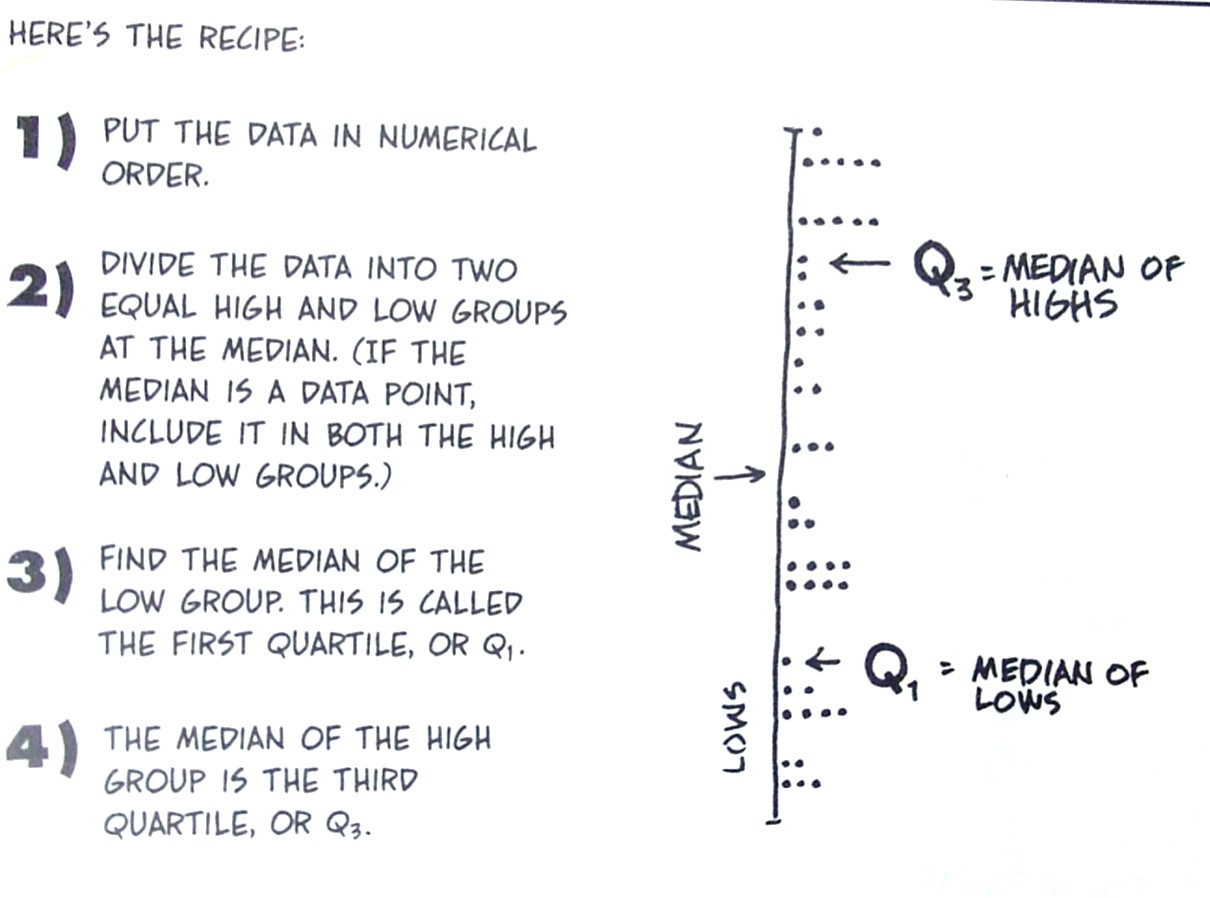
\includegraphics[width=0.4\linewidth]{fig/quartiles} \end{figure}
\end{frame}

\begin{frame}{When to use What}
\phantomsection\label{when-to-use-what}
\begin{itemize}
\tightlist
\item
  Use the \textbf{Mode} when the data are categorical:

  \begin{itemize}
  \tightlist
  \item
    \textbf{Mode}: is the value that occurs most frequently in your
    data.\\
  \item
    This is because having the same value occur for measurements with
    many significant digits is highly unlikely.
  \end{itemize}
\end{itemize}

\begin{itemize}
\tightlist
\item
  Use the \textbf{Median} when you have extreme scores:

  \begin{itemize}
  \tightlist
  \item
    \textbf{Median}: is simply the value that falls in the middle of all
    your data.
  \end{itemize}
\end{itemize}

\begin{itemize}
\tightlist
\item
  Use the \textbf{Mean} the rest of the time.
\end{itemize}

\begin{figure}
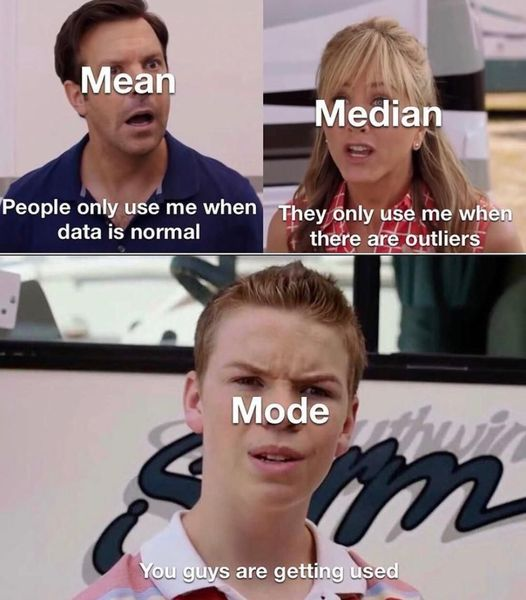
\includegraphics[width=0.25\linewidth]{fig/CnetralTendency} \end{figure}
\end{frame}

\begin{frame}{Variability}
\phantomsection\label{variability}
\begin{figure}
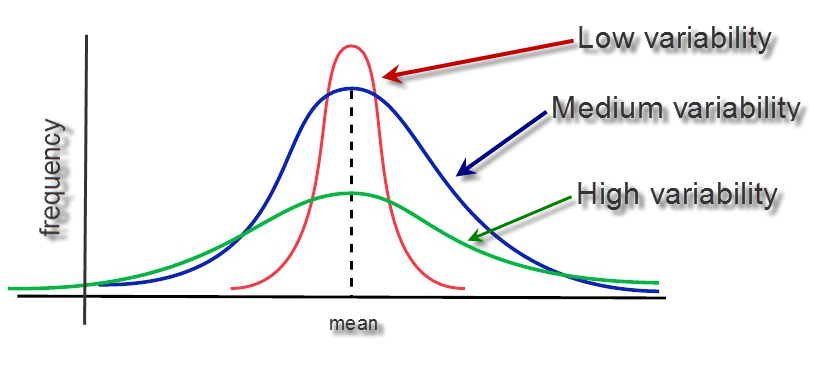
\includegraphics[width=0.25\linewidth]{fig/variability} \end{figure}
\end{frame}

\begin{frame}{Variability: Standard Deviation}
\phantomsection\label{variability-standard-deviation}
\begin{itemize}
\tightlist
\item
  Standard Deviation measures how spread out the numbers in a dataset
  are around the mean.
\end{itemize}

\begin{itemize}
\tightlist
\item
  The sample standard deviation \(s\) is calculated as:
  \[s = \sqrt{\frac{\sum_{i=1}^{n} (x_i - \bar{x})^2}{n - 1}}\]
\end{itemize}
\end{frame}

\begin{frame}{Variability}
\phantomsection\label{variability-1}
\begin{itemize}
\tightlist
\item
  \textbf{Variance} measures the average of the squared differences from
  the mean, indicating how spread out the data points are.
\end{itemize}

\begin{itemize}
\tightlist
\item
  The variance \(\sigma^2\) is calculated as:
  \[s^2 = \frac{\sum_{i=1}^{n} (x_i - \bar{x})^2}{n - 1}\]
\end{itemize}
\end{frame}

\begin{frame}{Variability: Range}
\phantomsection\label{variability-range}
\begin{itemize}
\tightlist
\item
  \textbf{Range} is the difference between the largest and smallest
  values in a dataset, providing a measure of the spread or dispersion
  of the data.
\end{itemize}

\begin{itemize}
\tightlist
\item
  The range is calculated as:
  \[\text{Range} = \text{max}(x) - \text{min}(x)\]
\end{itemize}
\end{frame}

\begin{frame}{Percentiles are useful for spread too}
\phantomsection\label{percentiles-are-useful-for-spread-too}
\begin{itemize}
\item
  You can use percentiles to get a feel for how spread out the data is
  and where most of your observations are contained:

  \begin{itemize}
  \tightlist
  \item
    Inter-quartile range (IQR) = Q3 -- Q1
  \end{itemize}
\end{itemize}
\end{frame}

\begin{frame}{Identifying outliers}
\phantomsection\label{identifying-outliers}
\begin{itemize}
\tightlist
\item
  An outlier is an observation that lies outside the overall pattern of
  a distribution (Moore and McCabe 1999).
\end{itemize}

\begin{itemize}
\tightlist
\item
  Usually, the presence of an outlier indicates some sort of problem.
  (e.g.~an error in measurement or sample selection).
\end{itemize}

\begin{itemize}
\tightlist
\item
  But they may also be an indicator of novel data or identification of
  unique and exciting observations.
\end{itemize}
\end{frame}

\begin{frame}{Identifying outliers}
\phantomsection\label{identifying-outliers-1}
\begin{itemize}
\tightlist
\item
  The first and third quantiles (Q1 and Q3) are often calculated to
  identify outliers.
\end{itemize}

\begin{itemize}
\tightlist
\item
  One method for systematically identifying outliers uses:

  \begin{itemize}
  \tightlist
  \item
    Q1 - (1.5 * the inter-quartile range)
  \item
    Q3 + (1.5 * the inter-quartile range)
  \end{itemize}
\end{itemize}

\begin{itemize}
\tightlist
\item
  Others identify outliers as any values below the 0.5th or above the
  99.5th percentile.
\end{itemize}
\end{frame}

\begin{frame}{When to use What}
\phantomsection\label{when-to-use-what-1}
\begin{itemize}
\tightlist
\item
  Use the \textbf{Standard deviation (SD)} in most cases.

  \begin{itemize}
  \tightlist
  \item
    SD quantifies how far, on average, each observation is from the
    mean.
  \item
    The larger the SD, the more highly variable your data.
  \end{itemize}
\end{itemize}

\begin{itemize}
\tightlist
\item
  Use \textbf{range (R)} when describing predictive models.

  \begin{itemize}
  \tightlist
  \item
    R is simply the maximum minus the minimum value in your data set
  \item
    R is important when modeling or making predictions, since your
    algorithms are valid only over the range of values used to calibrate
    your predictive model
  \end{itemize}
\end{itemize}

\begin{itemize}
\tightlist
\item
  Use the \textbf{IQR} to identify and test potential outliers in your
  data.
\end{itemize}
\end{frame}

\begin{frame}{Skewness}
\phantomsection\label{skewness}
\begin{itemize}
\tightlist
\item
  Skewness: This metric quantifies how balanced (symmetrical) your
  distribution curve is.
\end{itemize}
\end{frame}

\end{document}
